\documentclass{article}
\usepackage{tikz}
\usetikzlibrary{arrows.meta}
\begin{document}
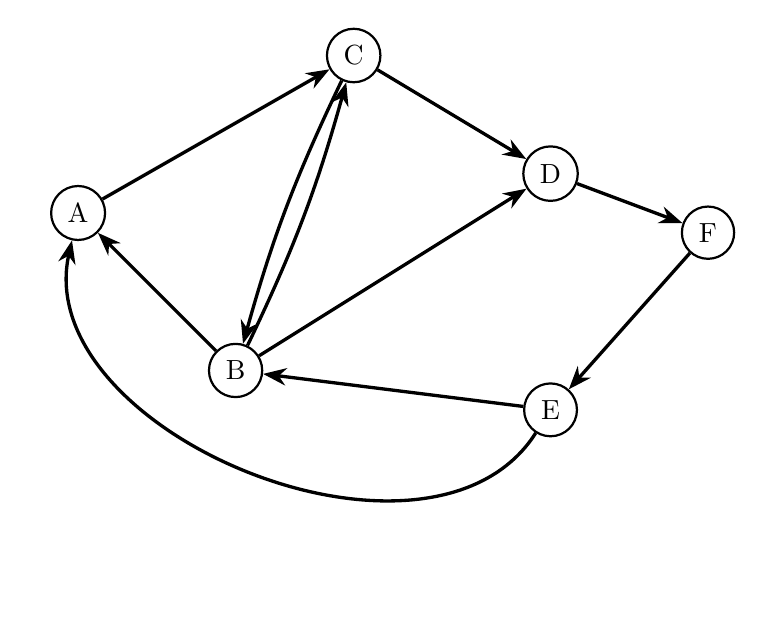
\begin{tikzpicture}
	\begin{scope}[every node/.style={circle,thick,draw}]
		\node (A) at (0,0) {A};
		\node (B) at (2,-2) {B};
		\node (C) at (3.5,2) {C};
		\node (D) at (6,0.5) {D};
		\node (E) at (6,-2.5) {E};
		\node (F) at (8,-0.25) {F} ;
	\end{scope}

	\begin{scope}[>={Stealth[black]},
		every node/.style={fill=white,circle},
		every edge/.style={draw=black,very thick}]
		\path [->] (A) edge (C);

		\path [->] (B) edge (A);
		\path [->] (B) edge[bend right=5] (C);
		\path [->] (B) edge (D);

		\path [->] (C) edge[bend right=5] (B);
		\path [->] (C) edge (D);

		\path [->] (D) edge (F);

		\path [->] (E) edge (B);
		\path [->] (E) edge[bend left=80] (A);

		\path [->] (F) edge (E);
	\end{scope}
\end{tikzpicture}
\vspace*{0.5em}

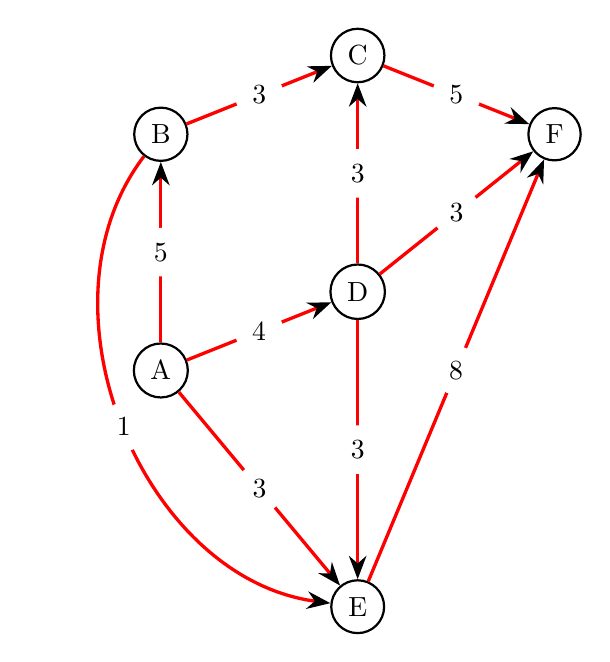
\begin{tikzpicture}
	\begin{scope}[every node/.style={circle,thick,draw}]
		\node (A) at (0,0) {A};
		\node (B) at (0,3) {B};
		\node (C) at (2.5,4) {C};
		\node (D) at (2.5,1) {D};
		\node (E) at (2.5,-3) {E};
		\node (F) at (5,3) {F} ;
	\end{scope}


	\begin{scope}[>={Stealth[black]},
		every node/.style={fill=white,circle},
		every edge/.style={draw=red,very thick}]
		\path [->] (A) edge node {$5$} (B);
		\path [->] (B) edge node {$3$} (C);
		\path [->] (A) edge node {$4$} (D);
		\path [->] (D) edge node {$3$} (C);
		\path [->] (A) edge node {$3$} (E);
		\path [->] (D) edge node {$3$} (E);
		\path [->] (D) edge node {$3$} (F);
		\path [->] (C) edge node {$5$} (F);
		\path [->] (E) edge node {$8$} (F);
		\path [->] (B) edge[bend right=60] node {$1$} (E);
	\end{scope}
\end{tikzpicture}

\end{document}